%!TEX TS-program = xelatex
%!TEX encoding = UTF-8 Unicode
%!BIB TS-program = biber
%!BIB program = biber

\documentclass[xetex,compress,spanish,xcolor=dvipsnames]{beamer}

%\setbeameroption{show notes}
\usepackage{pgfpages}\setbeameroption{show notes on second screen=right}
%\setbeameroption{show only notes}
%\setbeameroption{hide notes}

\mode<presentation>
{
  \usetheme{Warsaw}
  \usecolortheme[rgb={.7,.2,.2}]{structure}
  \setbeamercovered{transparent=50}
  \useoutertheme[footline=authortitle,subsection=false]{miniframes}
}
  \setbeamercovered{transparent=50}

\usepackage[no-math]{fontspec}
\usepackage[spanish,es-tabla,es-noshorthands,es-ucroman]{babel}
\usepackage{xltxtra}
\usepackage{fontspec}
\usepackage{xunicode}
\usepackage{amsmath}
\usepackage{amsthm}
\usepackage{graphicx}
\usepackage{amssymb}
\usepackage{hyperref}
\usepackage{siunitx}
\usepackage{tikz}
\usetikzlibrary{calc}
\usepackage{booktabs}
\usepackage{subfigure}
\usepackage{csvsimple}
\usepackage[colorinlistoftodos, shadow]{todonotes}
  \presetkeys{todonotes}{inline}{}

%% bib %%
\usepackage[style=authoryear,natbib=true,%
maxbibnames=99,maxcitenames=2,%
citestyle=authoryear-comp,doi=false,url=false,isbn=false,backend=biber,dashed=no,arxiv=false,eprint=false]{biblatex}
\bibliography{pfc-memoria.bib}
%% style %%
\defaultfontfeatures{Mapping=tex-text,Numbers={OldStyle}}
\setmainfont[Mapping=tex-text]{Hoefler Text}
\setromanfont[Mapping=tex-text]{Hoefler Text}
\setsansfont[Scale=MatchLowercase,Mapping=tex-text]{Gill Sans}
\setmonofont[Scale=0.9]{Courier New}
\sisetup{output-decimal-marker={,},
	product-units=single,
	detect-all, detect-inline-family=text, detect-inline-weight=text,
  detect-display-math=true}

%% custom macros %%
\newcommand{\email}[1]{%
  \href{mailto:#1}{\nolinkurl{<#1>}}}

\DeclareSIUnit[number-unit-product = {\,}]
	\pixel{px}

\usepackage{pifont}% http://tex.stackexchange.com/questions/42619/x-mark-to-match-checkmark
\newcommand{\cmark}{{\color{OliveGreen}\ding{51}}}
\newcommand{\xmark}{{\color{red}\ding{55}}}

%% doc info %%
\title{Procesamiento del Lenguaje Natural Aplicado al Análisis del Sentimiento de Opiniones}
\author[Guillermo Gutiérrez-Herrera]{Proyecto Fin de Carrera\\Ingeniero en Informática (Plan 97)\\[1em]
Realizado por: Guillermo Gutiérrez-Herrera\\[1em]
Dirigido por: José Antonio Troyano}
\institute{Departamento de Lenguajes y Sistemas Informáticos\\
Escuela Técnica Superior de Ingeniería Informática\\
Universidad de Sevilla}
\date{Septiembre de 2015}
\logo{
\includegraphics[width=10pt]{logo-lsi}\hspace{2pt}
\includegraphics[width=15pt]{logo-us}}
\subject{Procesamiento de NLP aplicado al Análisis de Sentimiento}
\keywords{Natural Language Processing, Machine Learning, Sentiment Analysis}


\expandafter\def\expandafter\insertshorttitle\expandafter{%
  \insertshorttitle\hfill%
  \insertframenumber\,/\,\inserttotalframenumber}

%% documento %%
\begin{document}

\frame{
\titlepage

\tikz[overlay,remember picture]
\node[anchor=center] at ($(current page.south west)+(1.3,1.3)$) {

\includegraphics[width=40pt]{logo-us}
};

\tikz[overlay,remember picture]
\node[anchor=center] at ($(current page.south west)+(2.9,1.3)$) {

\includegraphics[width=30pt]{logo-lsi}
};

\note{Buenas tardes. Mi nombre es Guillermo Gutiérrez y voy a presentar mi Proyecto Fin de Carrera titulado \emph{Procesamiento del Lenguaje Natural Aplicado al Análisis del Sentimiento de Opiniones}, que ha sido dirigido por el profesor José Antonio Troyano.}
}

%\section[Índice]{}
\frame{\frametitle{Índice}
\tableofcontents

\note[item]<1>{Empezaremos la presentación con una breve introducción y los objetivos del proyecto; y la planificación y metodología utilizados para su realización.}
\note[item]<1>{En la siguiente parte mostraremos los principales aspectos del procesamiento de lenguaje natural y aprendizaje automático que se estudian y describen en la memoria.}
\note[item]<1>{A continuación presentamos el problema concreto de clasificación automática del sentimiento; y el diseño de la solución propuesta.}
\note[item]<1>{Y por último las conclusiones del proyecto y un resumen de la bibliografía utilizada.}
}

\section[Introducción]{Introducción y objetivos}

\frame{\frametitle{Introducción}
\color{black}
En este proyecto se realiza
\begin{itemize}
\item Un estudio de investigación sobre
\begin{itemize}
\item Procesamiento de Lenguaje Natural (NLP)
\item Aprendizaje Automático (ML)
\end{itemize}
\item Una aplicación para experimentar con un problema de clasificación automática del sentimiento.
\end{itemize}

\note[item]<1>{El proyecto se compone de dos partes:}
\note[item]<1>{En la primera parte se realiza un estudio de investigación, con la lectura y análisis de amplia bibliografía en los ámbitos del lenguaje natural y aprendizaje automático.}
\note[item]<1>{Y en la segunda parte se pone en práctica estos conocimientos adquiridos con el desarrollo de una aplicación para la clasificación automática del sentimiento de opiniones.}
}

\frame{\frametitle{Objetivos}
\color{black}
Los objetivos del proyecto son
\begin{itemize}
\item Estudiar y explicar
\begin{itemize}
\item Diferencias entre el lenguaje natural y formal.
\item Estrategias, métodos, procedimientos y algoritmos para analizar y extraer información de textos en lenguaje natural (NLP).
\item Algoritmos de aprendizaje automático (ML).
\end{itemize}
\item Desarrollar
\begin{itemize}
\item Biblioteca unificada de NLP y ML para el análisis del sentimiento.
\item Aplicación gráfica para usar en el aula.
\end{itemize}
\end{itemize}

\note[item]<1>{Resumiendo, los objetivos son los siguientes:}
\note[item]<1>{Estudiar y explicar en la memoria la definión de lenguaje, los tipos de lenguaje y las características que los diferencian, entre en el lenguaje natural, lenguaje formal y lenguaje artificial o construido.}
\note[item]<1>{Explicar en la memoria las estrategias y algoritmos para el preprocesamiento, análisis y extracción de información a partir de los textos en lenguaje natural.}
\note[item]<1>{Estudiar y explicar con ejemplos, algunos métodos y algoritmos de aprendizaje automático aplicados a la extracción del conocimiento sobre las estructuras y la semántica del lenguaje natural; mostrando la manera de usar los corpus de texto existentes disponibles libremente en Internet como base para realizar este aprendizaje estadístico supervisado.}
\note[item]<1>{El cuarto objetivo es desarrollar una biblioteca que combine estos métodos de NLP y ML para el análisis del sentimiento.}
\note[item]<1>{Y por último una aplicación gráfica de escritorio para guiar al alumno durante todo el proceso de entrenamiento y clasificación del sentimiento.}
}

\section[Planificación]{Planificación y metodología}

\frame{%\frametitle{Planificación. Listado de tareas}
\color{black}
\centering
\begin{minipage}{0.68\textwidth}
\resizebox{0.80\textheight}{!}{\csvautotabular{gantt.csv}}
\end{minipage}
\begin{minipage}{0.25\textwidth}
\begin{tabular}{c|c}
\toprule
Estimado & 561 horas\\
Real & 625 horas\\
\bottomrule
\end{tabular}
\end{minipage}

\note[item]<1>{Ésta es una tabla de las tareas y horas planificadas para realizar el proyecto.}
\note[item]<1>{Los principales retrasos se debieron al estado de implementación de los frameworks declarativos de desarrollo rápido de aplicaciones utilizados durante la ejecución del proyecto:}
\note[item]<1>{Se usó en un primer momento Kivi, que es un framework que no estaba lo suficientemente maduro para su uso con Python 3, y después de varios problemas encontrados lo cambiamos por Qt.}
\note[item]<1>{Y usando Qt declarativo versión 5 también encontramos escasa la implementación de un control de tabla de datos que tuve que ampliar reimplementando una clase de Qt en Python 3.}
}

\frame{%\frametitle{Planificación. Diagrama de Gantt}
\tikz[overlay,remember picture]
\node[anchor=north west] at ($(current page.north west)+(-10pt,-8pt)$) {
  \pgfimage[width=1.03\paperwidth]{gantt}
};

\note[item]<1>{Aquí se puede ver la planificación a lo largo del calendario en un diagrama de gantt, con la lista de tareas en orden.}
\note[item]<1>{Se ha supuesto un trabajo diario de 8 horas en semanas de 5 días.}
}

\frame{\frametitle{Metodología de trabajo}
\begin{figure}[htbp]
\centering
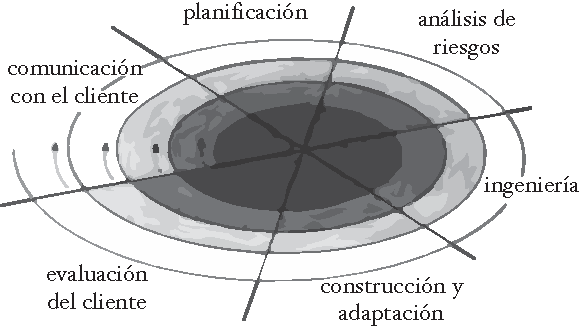
\includegraphics[width=0.58\textwidth]{espiral}
\caption[Modelo de ciclo de vida en espiral]{Modelo de ciclo de vida en espiral \citep{Boehm1988}}
\label{fig:espiral}
\end{figure}

\note[item]<1>{La metodología usada para organizar el trabajo y el desarrollo de la memoria y de la aplicación ha seguido la filosofía del modelo de ciclo de vida en espiral, con entregas al tutor por capítulos de la memoria y por iteraciones incrementales del software.}
}

\section{Investigación}

\frame{\frametitle{Investigación. NLP (I)}
\begin{itemize}
\item Diferenciar lenguaje a) natural, b) formal, c) construido
\item $1^\text{er}$ ejemplo: STUDENT, en LISP \citep{Bobrow1964}
\item Proceso de comunicación de 7 etapas \citep{Russell2003}
\item Jerarquía de Chomsky \citep{Chomsky1965}
\item Forma de trabajo usando \emph{corpus} (Linguistic Data Consortium)
\end{itemize}

\note[item]<1>{A partir de esta transparencia empezamos a enumerar los conceptos que se describen en la memoria.}
\note[item]<1>{Se explica la definición de los tres tipos de lenguajes: lenguaje natural para uso humano; lenguajes formales para uso en matemáticas y computación; y los lenguajes llamados construidos, artificiales o artísticos inventados.}
\note[item]<1>{Se muestra como ejemplo el programa STUDENT, tesis doctoral de Daniel Bobrow en 1964, como primer caso de utilización real del lenguaje natural, en este caso para la introducción de enunciados de problemas algebraicos que el programa pretendía resolver.}
\note[item]<1>{Comentamos también el proceso de Russell y Norvig, de las 7 etapas de comunicación de un mensaje entre dos personas desde que el emisor piensa lo que quiere comunicar hasta lo que el receptor comprende.}
\note[item]<1>{También se describe la jerarquía de Chomsky, diferenciando la capacidad expresiva de cada uno de los 4 niveles de la formalización de un lenguaje.}
}

\frame{\frametitle{Investigación. NLP (y II)}
\begin{enumerate}
\item Tokenización: \texttt{of escapades demonstrating the adage}  $\rightarrow$ \texttt{['of', 'escapades', 'demonstrating', \ldots]}
\item Expansión de contracciones: \texttt{hasn't} $\rightarrow$ \texttt{has not}
\item Supresión de \emph{stopwords}: \texttt{escapades demonstrating adage}
\item Radicación o \emph{stemming}: \texttt{escapades} $\rightarrow$ \texttt{escapade} \citep{Porter1980}
\item Lematización: \texttt{demonstrating}$\rightarrow$ \texttt{demonstrate} (tesauros, WordNet, word2vec, \citep{Handler2014})
\item Parte de la oración \emph{(part-of-speech)}: \texttt{of/IN escapades/NNS demonstrating/VBG the/DT adage/NN} \citep{Nebrija1492}
\item Análisis sintáctico:\\
{\centering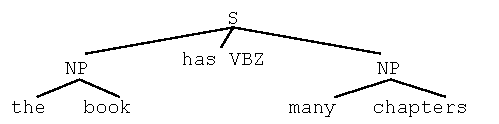
\includegraphics[height=1.8cm]{parsetree}}
\end{enumerate}

\note[item]<1>{Después de formalizar las características de los lenguajes, empezamos con el preprocesamiento, que son las transformaciones al texto que se pueden utilizar dependiendo del caso de aplicación.}
\note[item]<1>{En la memoria se describe el proceso de división en tokens, expansión de contracciones en el caso del inglés, supresión de palabras vacías de significado, el algoritmo de radicación de Martin Porter, el reemplazo por el lema principal de la palabra, la anotación gramatical (artículo, sustantivo, adjetivo, verbo), y el análisis sintáctico de las oraciones.}
\note[item]<1>{No hay que utilizar siempre todos los pasos, depende de la calidad del texto del corpus empleado y de lo que se desee extraer de ellos.}
}

\frame{\frametitle{Investigación. ML}
\begin{itemize}
\item Concepto del problema de clasificación automática \citep{Manning2008}
\item Tipologías a) supervisado, b) no supervisado, c) semi-supervisado
\item Extracción de características a partir del texto: $n$-gramas, RNN, VM-RNN \citep{Socher2013}
\item Reducción de características
\item Estimadores: Naïve Bayes Multinomial/Gausiano, LDA/QDA, SVM \citep{Jurafsky2015,Ruiz2001,Pedregosa2011,Russell2009}
\item Medida del rendimiento del estimador \citep{Perkins2010}
\end{itemize}

\note[item]<1>{Luego pasamos a dar un repaso de los tipos de aprendizaje automático de inteligencia artificial: supervisado, no supervisado y supervisado; enfocados a resolver el problema de clasificación automática de muestras.}
\note[item]<1>{También comentamos algunas formas de extraer características a partir de los corpus de texto, como son el conteo de la distribución de n-gramas, o las redes neuronales recursivas basadas en el árbol del análisis sintáctico de las frases publicado por Socher en 2013.}
\note[item]<1>{Se describe el funcionamiento de algunos estimadores estadísticos y la forma de comparar su rendimiento.}
}


\section{Problema}

\frame{\frametitle{Polaridad del sentimiento}
\begin{definition}[Polaridad del sentimiento]
Es la conclusión que se extrae de la comprensión de un documento de tipo crítico: si el objeto de la crítica es bueno (sentimiento positivo) o malo (resp., negativo).
\end{definition}
\begin{figure}
\centerline{\pgfimage[height=0.47\textheight]{tramos-polaridad}}
\caption{Escala de valoración del sentimiento usada en Penn Sentiment Treebank de la Universidad de Pennsylvania \citep{Socher2014}}
\end{figure}

\note[item]<1>{Pasamos a describir el problema que vamos a resolver con la aplicación desarrollada. Se trata de una competición de Kaggle.com, una web que se dedica a proponer retos sobre ciencia de datos (data science).}
\note[item]<1>{En este caso se trata de extraer un modelo de clasificación automática del sentimiento de opiniones, usando para ello un dataset de críticas de cine etiquetado con su sentimiento, es decir, si la crítica es positiva o negativa.}
\note[item]<1>{Para producir este dataset se extrae el texto de las críticas de la página web de Rotten Tomatoes, se parsean en unidades más pequeñas y varios voluntarios se encargan de asociar a cada frase un sentimiento.}
\note[item]<1>{Este dataset es el que forma parte del estudio realizado por Socher dentro del proyecto para el análisis del sentimiento en la Universidad de Pennsylvania.}
\note[item]<1>{Los voluntarios clasificaban el sentimiento en una escala con 35 graduaciones, que luego se agruparon en 5 clases (muy negativo, negativo, neutro, positivo y muy positivo).}
}

\frame{\frametitle{Problema a resolver}
\begin{itemize}
\item Problema de clasificación supervisado
\item Clases: $[0:4] \rightarrow [--,-,0,+,++]$
\item Entrada: corpus de Rotten Tomatoes \citep{Pang2005} \\
\centerline{\footnotesize
\begin{tabular}{llp{5cm}l}\toprule
PhraseId & SentenceId & Phrase & Sentiment \\ \midrule
1 & 1 & A series of escapades demonstrating the adage that what is good for the goose is also good for the gander , some of which occasionally amuses but none of which amounts to much of a story . & 1 \\
2 & 1 & A series of escapades demonstrating the adage that what is good for the goose & 2 \\ \bottomrule
\end{tabular}
}
\item Salida: clasificación del sentimiento
\end{itemize}

\note[item]<1>{Es un problema de clasificación supervisado, con 5 clases, cuya entrada es una tabla que tiene esta forma, con la que se realiza el entrenamiento.}
\note[item]<1>{Una vez entrenado se clasifica el subconjunto de evaluación al que le falta la columna de clase, que es lo que el modelo entrenado tiene que predecir.}
}



\section[Diseño]{Diseño de la solución}

\frame{\frametitle{Diseño de la solución}
\noindent
\begin{figure}
\centerline{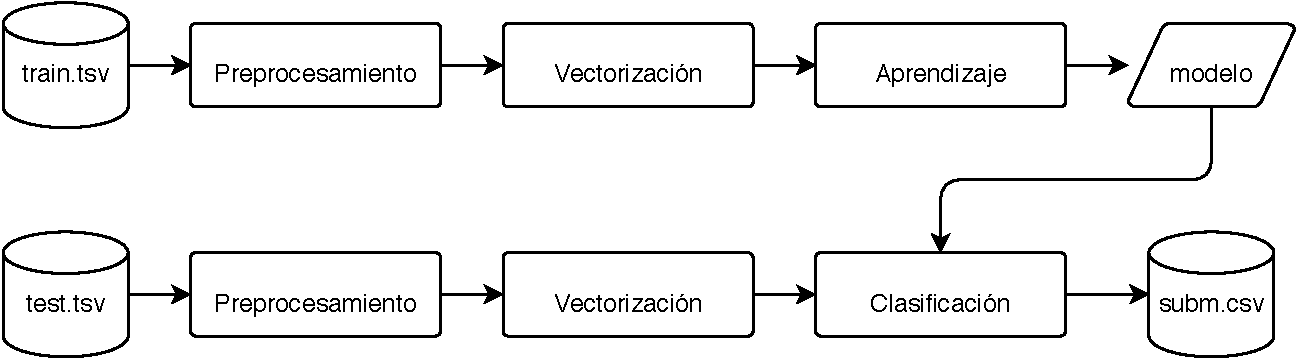
\includegraphics[width=0.95\paperwidth]{PFC-sent-anal-workflow.pdf}}
\caption{Fase de entrenamiento (arriba), fase de clasificación (abajo)}
\label{fig:PFC-sent-anal-workflow}
\end{figure}

\note[item]<1>{La solución propuesta divide el proceso en dos pasos, uno de entrenamiento y otro de clasificación, pero de manera integrada.}
\note[item]<1>{La tabla se lee y se preprocesa con las opciones que ha marcado el usuario; después el texto preprocesado se vectoriza usando las opciones de extracción de características. Esto da como resultado una matriz numérica n-dimensional con la que se entrena un modelo que aprendizaje con los ajustes selecionados por el usuario.}
\note[item]<1>{En la segunda fase se realiza sobre el subconjunto de evaluación, el mismo preprocesamiento y vectorización usados en el entrenamiento, y para la fase de clasificación se usa uno de los modelos previamente entrenados, obteniendo el resultado con las predicciones.}
}


%\frame{\frametitle{Diseño. Patrón de diseño}
%\color{black}
%\begin{figure}
%\centerline{
%\begin{minipage}{0.48\paperwidth}
%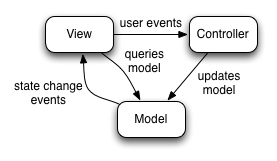
\includegraphics[width=\textwidth]{MVC}
%\end{minipage}
%\begin{minipage}{0.48\paperwidth}
%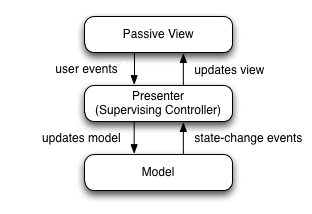
\includegraphics[width=\textwidth]{MVP}
%\end{minipage}
%}
%\caption{Patrones de diseño MVC y MVP}
%\label{fig:patrones-diseno}
%\end{figure}
%{\footnotesize \url{http://www.gwtproject.org/articles/testing_methodologies_using_gwt.html}}
%
%\note[item]<1>{...}
%}

\frame{\frametitle{Diseño. Arquitectura de componentes}
\centerline{\resizebox{!}{0.75\paperheight}{\input{architecture.puml.tex}}}

\note[item]<1>{La arquitectura del sistema mezcla distintos componentes en Python 3 y en C++, organizados en un patrón de diseño Modelo-Vista-Presentador.}
\note[item]<1>{Se implementan dos módulos Python. El módulo de modelo utiliza las bibliotecas de scikit-learn para el aprendizaje automático, y de NLTK3 para el procesamiento de texto, encargándose de orquestar todo el proceso de aprendizaje y clasificación.}
\note[item]<1>{El módulo en la presentación se encarga de mostrar visualmente los datos y la ventana que hace de interfaz con el usuario, usando para ello la biblioteca de Qt5 y el motor del lenguaje declarativo QML y su envoltorio para Python.}
}

%\frame{\frametitle{Diseño. Toolkits de desarrollo GUI}
%\todo{Comentar Kivi, comentar QML(Qt)}
%
%\note[item]<1>{...}
%}

\frame{\frametitle{Diseño. Pantallas}

\centerline{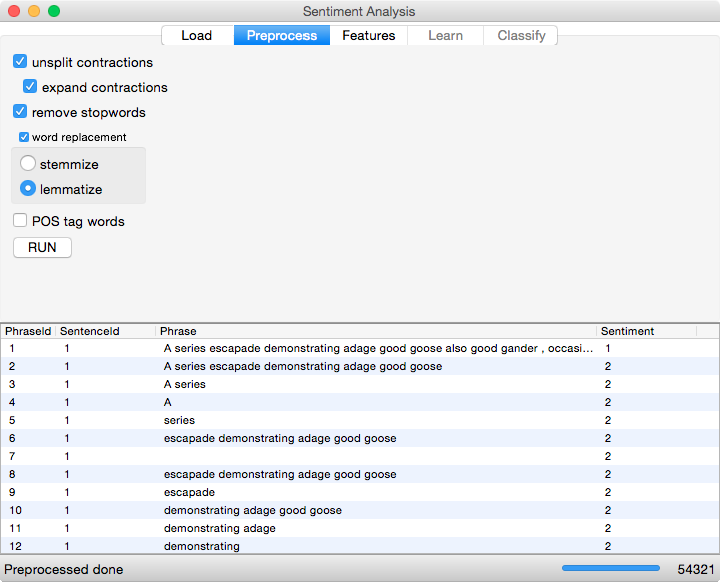
\includegraphics[width=0.9\textwidth]{ss-04-preproc-tab}}

\note[item]<1>{La pantalla de la aplicación tiene esta forma, está organizada por pestañas en orden de izquierda a derecha, mostrando un panel para realizar los ajustes de la etapa.}
\note[item]<1>{Al terminar cada etapa se muestra una tabla con el resultado.}
}


\section[Conclusiones]{Conclusiones y continuidad}

\frame{\frametitle{Conclusiones}
\color{black}
Se han conseguido los objetivos propuestos
\begin{itemize}
\item[\cmark] Estudio y análisis de bibliografía sobre NLP y ML.
\item[\cmark] Desarrollo de la aplicación multiplataforma para la experimentación en clasificación automática de sentimiento.
\end{itemize}

\note[item]<1>{Las conclusiones son que te han conseguido los objetivos marcados, el estudio de NLP y ML y la manera de combinarlos.}
\note[item]<1>{Y el desarrollo de la aplicación para poder experimentar con los algoritmos.}
}

\frame{\frametitle{Posibles mejoras}

\begin{itemize}
\item Exportación del modelo aprendido
\item Añadir más métodos de aprendizaje
\item Añadir más métodos de extracción de características
\end{itemize}

\note[item]<1>{Como posibles mejoras futuras que se podrían hacer se propone la posibilidad de exportar en un fichero el modelo aprendido,}
\note[item]<1>{añadir otros métodos de aprendizaje,}
\note[item]<1>{y otros métodos de extracción de características.}
}

\section{Bibliografía}

\frame[allowframebreaks]{\frametitle{Bibliografía}

\setsansfont[Scale=0.6,Mapping=tex-text]{Gill Sans}
\printbibliography[heading=none,title=\bibname]
\setsansfont[Scale=MatchLowercase,Mapping=tex-text]{Gill Sans}

\note[item]<1>{Esta es una muestra de la bibliografía empleada en el proyecto, en total unas 60 referencias.}
}

\appendix

\frame{
\color{black}
\Huge ¿Preguntas?
\tikz[overlay,remember picture]
\node[anchor=center] at ($(current page.center)+(2,0)$) {
  
\includegraphics[width=120pt]{preguntas}
};

\note[item]<1>{Y nada más, muchas gracias, y si tienen alguna pregunta.}
}

\frame{
\color{black}
\centering
\huge Gracias por su atención

\vspace{0.2\textheight}

\normalsize
\begin{minipage}{5.3cm}
Guillermo Gutiérrez-Herrera

\email{guiguther@alum.us.es}

\email{xiterrex@gmail.com}
\end{minipage}

\note[item]<1>{...}
}

\end{document}
